\section{Introduction}
We are interested in designing autonomous systems to perform complex
mobile manipulation tasks over long time horizons (e.g., setting a
dinner table, doing laundry). We approach this problem in the
framework of combined \emph{task and motion planning} ({\sc tamp}).

In {\sc tamp}, an agent is given a symbolic, logical characterization
of actions (e.g., move, grasp, putdown), along with a geometric
encoding of the environment.  Efficient integration of high-level,
symbolic task planning and low-level, geometric motion planning is
difficult; recent research has proposed several
approaches~\cite{srivastava2014combined, deardenplanningtamp,
  kaelbling2011hierarchical, lagriffoul2014orientation, GarrettWAFR14,
  dornhege2012semantic}.  In this paper, we adopt the abstraction
framework developed by Srivastava et al.~\cite{srivastava2014combined}
(henceforth referred to as {\sc sfrcra-14}) to factor the reasoning
and search problems into interacting logical and geometric components.

\begin{figure}[t]
  \centering
    \noindent
    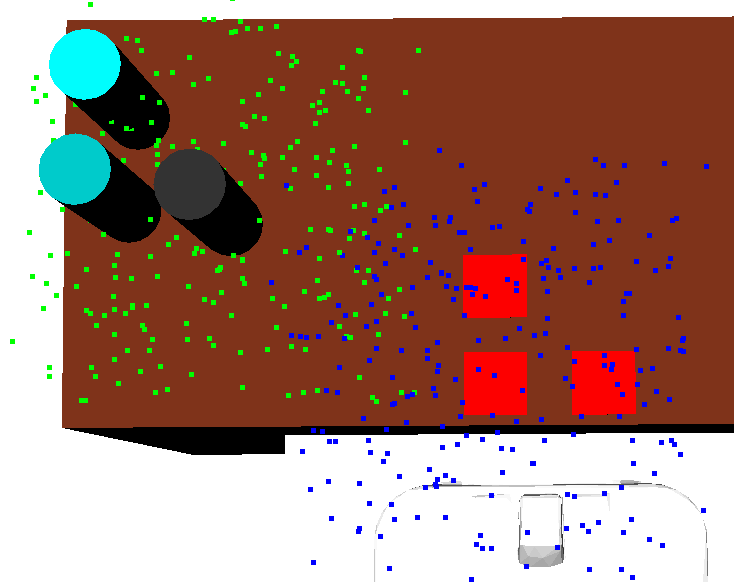
\includegraphics[scale=0.112]{images/learns.png}
    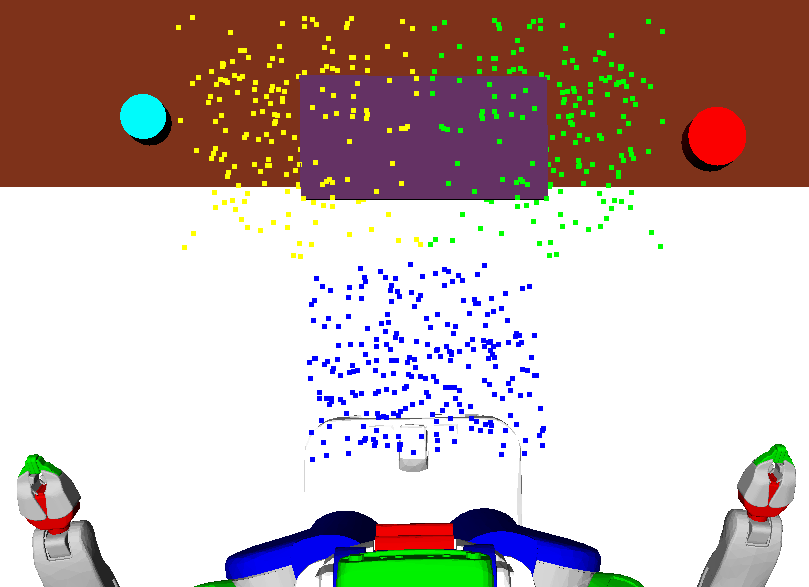
\includegraphics[scale=0.13]{images/dinner_tray_initial.png}
    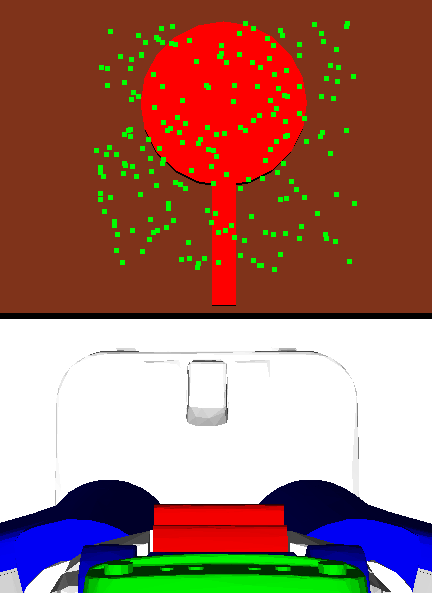
\includegraphics[scale=0.13]{images/frying_initial.png}\vspace{1em}
    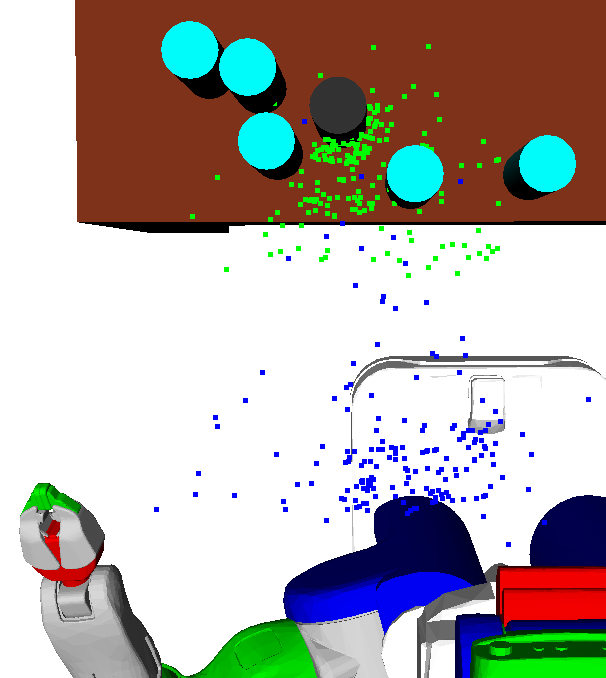
\includegraphics[scale=0.112]{images/learn12.png}
    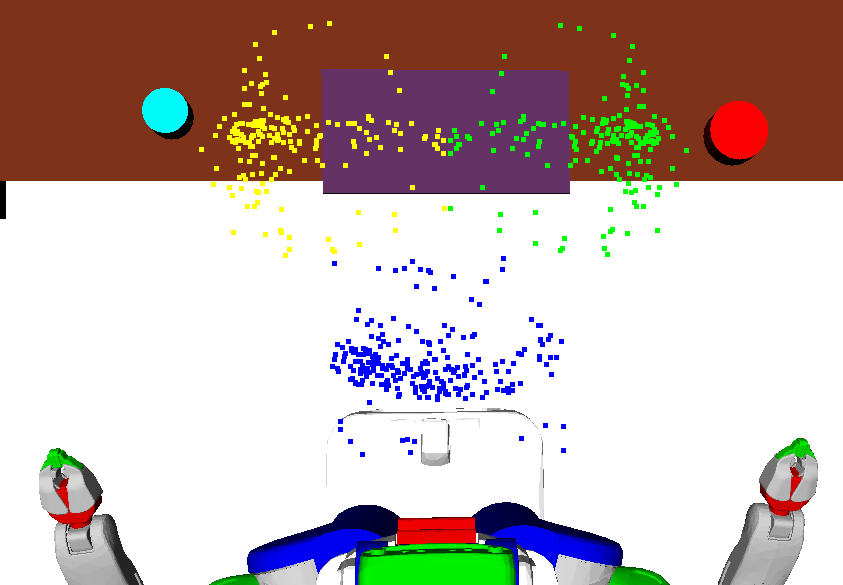
\includegraphics[scale=0.13]{images/dinner_tray_final.png}
    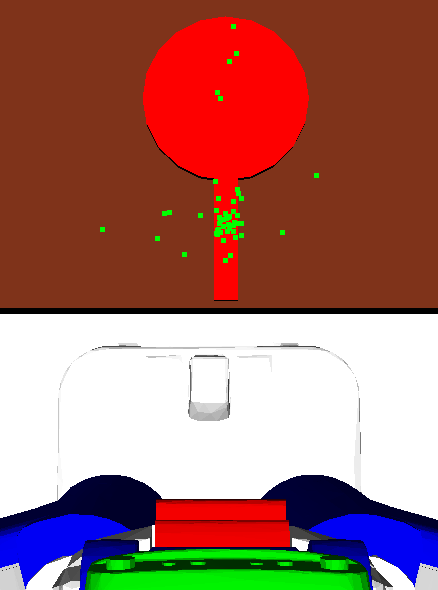
\includegraphics[scale=0.13]{images/frying_final.png}
  \caption{\small{We apply reinforcement learning to speed up planning
      for {\sc tamp} tasks. We break the problem down into a low-level
      policy that samples promising values for continuous parameters
      (e.g., pre-grasp poses, grasps, \ldots etc.), and a high-level
      policy that ranks different high-level plans. The above figures
      illustrate learning for the low-level system. The top images
      show initial, uniform distributions. The bottom images show
      learned distributions over base pose (blue) and end effector
      pose (green, yellow) for pick tasks in our simulated domains: a
      can (left), a tray (middle), and a frying pan (right).  The
      green and yellow points refer to the positions of the tool
      center points; the end effectors are oriented to point toward
      the object being grasped. The can and frying pan are picked up
      using only one gripper.}}
  \label{fig:cover}
\end{figure}

In this work, we develop a complete algorithm for {\sc tamp} and
propose learning methods to guide a joint search in the space of
high-level, symbolic plans and their low-level \emph{refinements}:
instantiations of continuous values for symbolic references in the
plan. For example, in a pick-place domain, a high-level plan consists
of a sequence of move, grasp, and putdown actions, while its
refinement is a sequence of collision-free trajectories that implement
the plan. We refer to the search for a valid refinement as \emph{plan
  refinement}.

{\sc sfrcra-14} uses error information propagated from the geometric
planner to update the symbolic state and generate a new high-level
plan.  For example, if motion planning discovers an obstructionq in a
pick-place domain, the new plan may involve moving the obstruction out
of the way.  The key step in our approach defines a \emph{plan
  refinement graph}, where nodes are high-level plans and edges are
unsatisfiable preconditions the explain a failed attempt at
refinement. We develop a complete algorithm that interleaves search
over this graph with plan refinement.

Natrually, the space of task plans and their possible refinements is
quite large. To combat this, we present machine learning techniques
that guide search over both components of the search. At the low
level, our system learns to propose continuous values for symbolic
references that are likely to result in collision-free
trajectories. Discretizing the space of continuous parameters is a
common step in {\sc tamp} systems and largely relies on hand-coded
heuristics or well-chosen sampling distributions. 

We apply reinforcement learning ({\sc rl}) to learn domain-specific
distributions over these values in a domain-independent fashion.  Our
approach draws inspiration from Zhang and
Dietterich~\cite{JobShopSched}, who applied {\sc rl} to job shop
scheduling. In their formulation, states correspond to schedules and
actions propose changes to the schedule. In our setting, states
correspond to (potentially infeasible) refinements and actions propose
new values for symbolic references.


At the high level, we train heuristics that estimate how difficult it
is to refine a given plan. Directly applying reinforcement learning to
this task is challenging because actions amount to either motion
planning or task planning, and so are time consuming, and because
there are often a wide range of options to select between. It is,
however, fairly easy for a person to determine high-level plans that
are promising, so we use inverse reinforcement learning based on
expert demonstrations to train heuristics for this problem.


The contributions of our work are as follows: 1) we present a complete
algorithm for {\sc tamp}; 2) we present a randomized local search
algorithm for plan refinement that is easily formulated as an {\sc
  mdp}; 3) we apply {\sc rl} to learn a policy for this {\sc mdp}; 4)
we learn from expert demonstrations to efficiently search the space of
high-level plans, given options that address different
infeasibilities; and 5) we run experiments to evaluate the performance
of our system in a variety of simulated domains. Our results
demonstrate significantly improved performance over {\sc sfrcra-14}.
